\section[Problèmes non-linéaires]{Problèmes non-linéaires}

\begin{frame}{Problèmes non-linéaires}
	Dans cette section on verra:
	\begin{itemize}
		\item Comment on peut adapter la définition d'un neurone artificiel pour le préparer à l'algorithme d'apprentissage de \textbf{rétro-propagation du gradient}.
		\item Comment on peut créer un \textbf{réseau} pour résoudre un problème non-linéaire.
		\item Comment on pourrait adapter la structure d'un neurone artificiel pour les problèmes de \textbf{régression}.
	\end{itemize}
\end{frame}

\subsection[Dérivabilité]{Dérivabilité}

\begin{frame}{De la fonction de Heaviside à la fonction logistique}
	L'algorithme de rétro-propagation du gradient, que l'on verra plus tard dans le cours, nécessite de calculer des \textbf{gradients}. La fonction de Heaviside possède des gradients \textbf{nuls} (quand ils existent). Cette particularité en fait un très mauvais choix pour les réseaux de neurones entraînés avec cette rétro-propagation du gradient. On lui préfère donc une fonction \textbf{logistique}:
	
	\begin{figure}
		\centering
		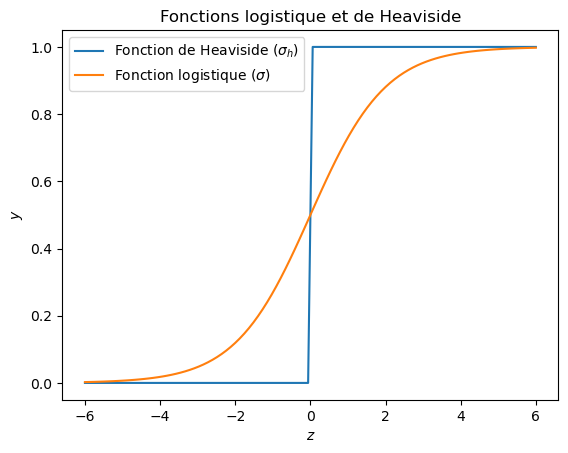
\includegraphics[height=0.4\linewidth]{Images/nonlinearites01}
		\label{fig:nonlinearites01}
	\end{figure}	
\end{frame}

\begin{frame}{Nouvelle formulation d'un neurone artificiel}
	Avec la fonction logistique, la formulation d'un neurone artificiel devient:
	
	\begin{equation*}
		y = \logistic{x \cdot w + b}
	\end{equation*}
	
	\pause
	\vspace{0.3cm}
	C'est \textbf{exactement} la formulation de la régression logistique ! La méthode de rétro-propagation du gradient permet de calculer les gradients de l'erreur de prédiction par rapport aux poids $w$ et au biais $b$. Une fois ces gradients obtenus, l'optimisation se réalise grâce à des \textbf{méthodes de descente de gradient}. Un tel neurone artificiel dispose donc de la même formulation que la régression logistique et du même algorithme d'apprentissage. C'est \textbf{rigoureusement} la même chose.
\end{frame}

\begin{frame}{Différence avec la régression logistique}
	La différence avec la régression logistique réside dans l'approche pour résoudre des problèmes non-linéairement séparables:
	\begin{itemize}
		\item La régression logistique utilise des augmentations différentes pour les caractéristiques d'entrée $X$ afin d'introduire des non-linéarités.
		\item Dans l'approche réseau de neurones, on joue principalement sur des \textbf{assemblages} de neurones en \textbf{réseau}.
	\end{itemize}
\end{frame}

\subsection[Architecture d'un réseau]{Architecture d'un réseau}

\begin{frame}{Un abus de langage usuel pour les réseaux de neurones}
	On écrit couramment l'expression suivante pour un empilement vertical des observations pour un neurone artificiel:
	
	\begin{equation*}
		Y = \logistic{X \cdot w + b}
	\end{equation*}
	
	Mais c'est un abus. En effet $X \in \mathcal{M}_{n,p}(\R)$, $Y \in \mathcal{M}_{n,1}(\R)$, $w \in \mathcal{M}_{p,1}(\R)$ et $b \in \R$. On ne peut rigoureusement pas additionner un vecteur et un scalaire.
	
	\vspace{0.2cm}
	\pause
	
	C'est une pratique qui nous vient du monde de l'informatique. Les librairies de calcul utilisent un concept de \textbf{broadcasting} qui permet de modifier automatiquement la forme d'une opérande entre vecteurs, matrices, tenseurs et scalaires. Rigoureusement, l'opération qui va être réalisée est la suivante:
	
	\begin{equation*}
		Y = \logistic{X \cdot w + b \cdot \mathbf{1}_n}
	\end{equation*}
	
	Avec $\mathbf{1}_n \in \mathcal{M}_{n,1}$ tel que $\mathbf{1}_n = \begin{pmatrix}
		1 & 1 & \cdots & 1
	\end{pmatrix}^T$.
\end{frame}

\begin{frame}{Assemblage de neurones en couches}
	Dans ce cours, on se limitera à des réseaux de neurones \textbf{denses}, aussi appelés \textbf{totalement connectés}. 
	
	\vspace{0.3cm}
	
	Ces réseaux font apparaitre des assemblages de neurones en \textbf{couches}. 
	
	\vspace{0.3cm}
	
	Un tel réseau est parfois aussi appelé \textbf{Perceptron Multicouche} en référence historique même si le neurone n'utilise plus de fonction de Heaviside comme fonction d'\textbf{activation} mais bien d'une fonction logistique.
\end{frame}

\begin{frame}{Assemblage de neurones en couches}
	Un empilement vertical des observations donnera la formulation suivante pour une couche de neurones:
	
	\begin{block}{Une couche de neurones dans un réseau dense}
		L'information se propage de la couche $k$: $X^{(k)}$ à la couche $k+1$: $X^{(k+1)}$ lors d'une \textbf{passe avant} dans le réseau de neurones. La dimensionnalité de $X$ change entre chaque couche: $X^{(k)} \in \mathcal{M}_{n,p^{(k)}}(\R)$ et $X^{(k+1)} \in \mathcal{M}_{n,p^{(k+1)}}(\R)$. Les \textbf{poids} des neurones dans la couche sont notés $W^{(k+1)} \in \mathcal{M}_{p^{(k)},p^{(k+1)}}(\R)$ et les \textbf{biais} sont notés $b^{(k+1)} \in \mathcal{M}_{1,p^{(k+1)}}(\R)$:
		\begin{equation*}
			X^{(k+1)} = \logistic{X^{(k)} W^{(k+1)} + b^{(k+1)}}
		\end{equation*}
		Attention: dans l'empilement vertical, les exposants $(k)$ et $(k+1)$ permettent d'identifier la couche du réseau et plus les observations.
	\end{block}
\end{frame}

\begin{frame}{Le broadcasting pour une couche de neurones}
	Encore une fois, la formule donnée sur la diapositive précédente est un abus de langage:
	
	\begin{equation*}
		X^{(k+1)} = \logistic{X^{(k)} W^{(k+1)} + b^{(k+1)}}
	\end{equation*}
	
	Dans cette expression, le produit $X^{(k)} W^{(k+1)}$ est une matrice de dimension $n \times p^{(k+1)}$ et $b^{(k+1)}$ est une vecteur ligne $1 \times p^{(k+1)}$. L'opération de broadcasting réalisée par un programme informatique est la suivante:
	
	\begin{equation*}
		X^{(k)} W^{(k+1)} + \left.
		\smash[b]{\underbrace{
				\begin{pmatrix}
					\text{---} & b^{(k+1)} & \text{---} \\
					\text{---} & b^{(k+1)} & \text{---} \\
					\vdots & \vdots & \vdots \\
					\text{---} & b^{(k+1)} & \text{---}
				\end{pmatrix}
			}_{p^{(k+1)} \text{ colonnes}}}
		\right\} n \text{ lignes}
		\vphantom{\underbrace{\begin{matrix} \\ \\ \\ \end{matrix}}_{p^{(k)} \text{ colonnes}}}
	\end{equation*}
	
\end{frame}

\begin{frame}{Architecture d'une couche de neurones}
	\begin{center}
		\resizebox{0.85\textwidth}{!}{
			\begin{tikzpicture}[x=1.5cm, y=1.2cm, >=Stealth]
				
				% --- Styles ---
				\tikzset{
					input/.style={circle, draw=black, minimum size=0.8cm, inner sep=0pt, font=\small},
					neuron/.style={circle, draw=black, minimum size=1cm, inner sep=0pt},
					weight/.style={font=\small, text=red!70!black, fill=white, inner sep=1pt, rounded corners}
				}
				
				% --- 1. Entrées (Inputs) ---
				\node[input] (x1) at (0, 3) {$x_1^{(k,i)}$};
				\node[input] (x2) at (0, 1.5) {$x_2^{(k,i)}$};
				\node (xdots) at (0, 0) {$\vdots$};
				\node[input] (xp) at (0, -1.5) {$x_{p^{(k)}}^{(k,i)}$};
				
				\node[anchor=south, font=\scriptsize\bfseries] at (x1.north) {Couche $X^{(k)}$};
				
				% --- 2. Zone Couche de Neurones ---
				\draw[dashed, gray!50, rounded corners=10pt, fill=blue!2] (2.2, -2.7) rectangle (5.5, 4.5);
				\node[font=\scriptsize\bfseries, text=gray!80!black] at (3.85, 4.2) {Couche Dense (3 neurones)};
				
				% --- 3. Création des Neurones ---
				\foreach \j/\y in {1/3, 2/0.75, 3/-1.5} {
					
					% Bloc de Somme
					\node[neuron, fill=white] (sum\j) at (3, \y) {$\displaystyle \sum$};
					
					% Bloc d'Activation (Logistique)
					\node[neuron, fill=white] (act\j) at (4.7, \y) {};
					
					% Dessin de la Sigmoïde (S-curve) dans le noeud
					\draw[thick, blue] ([xshift=-0.25cm, yshift=-0.25cm]act\j.center) 
					.. controls ([xshift=0.1cm, yshift=-0.25cm]act\j.center) and ([xshift=-0.1cm, yshift=0.25cm]act\j.center) .. 
					([xshift=0.25cm, yshift=0.25cm]act\j.center);
					
					% Transfert interne (z)
					\draw[->, thick] (sum\j) -- (act\j) node[midway, above, font=\small] {$z_{\j}^{(k+1,i)}$};
					
					% Sortie (y)
					\node (y\j) at (6.5, \y) {$x_{\j}^{(k+1,i)}$};
					\draw[->, thick] (act\j) -- (y\j);
					
					% Biais local pour la lisibilité
					\node[input, fill=green!10, draw=green!60!black, minimum size=0.4cm, font=\tiny] (b\j) at (3, \y+0.9) {$+1$};
					\draw[->, green!60!black, thick] (b\j) -- (sum\j) node[midway, right, font=\small] {$b_{\j}^{(k+1)}$};
				}
				
				\node[anchor=south, font=\scriptsize\bfseries] at (y1.north) {Couche $X^{(k+1)}$};
				\node[anchor=north, font=\small, text=blue, align=center] at (act3.south) {Logistique\\$\sigma(z)$};
				
				% --- 4. Connexions (Synapses) ---
				% Lignes de fond (grisées)
				\foreach \y in {1, 2, 3} {
					\draw[->, gray!40] (x1) -- (sum\y);
					\draw[->, gray!40] (x2) -- (sum\y);
					\draw[->, gray!40, dashed] (xdots) -- (sum\y);
					\draw[->, gray!40] (xp) -- (sum\y);
				}
				
				% Lignes mises en évidence pour montrer la notation
				\draw[->, gray!80, thick] (x1) -- (sum1) node[pos=0.25, above, weight] {$w_{1,1}^{(k+1)}$};
				\draw[->, gray!80, thick] (xp) -- (sum3) node[pos=0.25, below, weight] {$w_{3,p^{(k)}}^{(k+1)}$};
				
			\end{tikzpicture}
		}
	\end{center}
\end{frame}

\begin{frame}{Architecture d'un Perceptron Multicouche (MLP)}
	Afin de représenter un réseau complet, on simplifiera en faisant disparaître les biais. \`A partir de maintenant, dans le cours, un neurone noté $\Sigma$ dans la représentation ci-dessous représente à la fois la somme pondérée des entrées (poids) et le seuil (biais):
	\begin{center}
		\resizebox{1.0\textwidth}{!}{
			\begin{tikzpicture}[x=2cm, y=1.3cm, >=Stealth]
				
				% --- Styles ---
				\tikzset{
					input/.style={circle, draw=black, minimum size=0.8cm, inner sep=0pt, font=\small},
					sum/.style={circle, draw=black, minimum size=0.8cm, inner sep=0pt, fill=white},
					act/.style={circle, draw=blue!80, minimum size=0.8cm, inner sep=0pt, fill=blue!5},
					link/.style={->, red!70!black, opacity=0.4, thick},
					internal/.style={->, gray!60, thick}
				}
				
				% --- 1. Couche d'Entrée (3 entrées) ---
				\foreach \i in {1, 2, 3} {
					\node[input] (x\i) at (0, 4-\i*1.2) {$x_\i^{(i)}$};
				}
				\node[anchor=south, font=\scriptsize\bfseries] at (x1.north) {Entrées};
				
				% --- 2. Couche Cachée (3 neurones décomposés) ---
				\foreach \h in {1, 2, 3} {
					% Opérateur linéaire (Somme)
					\node[sum] (S\h) at (1.5, 4-\h*1.2) {$\sum$};
					% Opérateur non-linéaire (Activation)
					\node[act] (A\h) at (2.4, 4-\h*1.2) {};
					
					% Dessin de la Sigmoïde bleue
					\draw[thick, blue] ([xshift=-0.2cm, yshift=-0.15cm]A\h.center) 
					.. controls ([xshift=0.05cm, yshift=-0.15cm]A\h.center) and ([xshift=-0.05cm, yshift=0.15cm]A\h.center) .. 
					([xshift=0.2cm, yshift=0.15cm]A\h.center);
					
					% Lien interne entre somme et activation
					\draw[internal] (S\h) -- (A\h);
				}
				\node[anchor=south, font=\scriptsize\bfseries, text=gray] at (1.95, 3.2) {Couche Cachée};
				
				% --- 3. Couche de Sortie (1 neurone décomposé, centré verticalement) ---
				\node[sum] (So) at (3.5, 1.6) {$\sum$};
				\node[act] (Ao) at (4.0, 1.6) {};
				
				% Dessin de la Sigmoïde bleue pour la sortie
				\draw[thick, blue] ([xshift=-0.2cm, yshift=-0.15cm]Ao.center) 
				.. controls ([xshift=0.05cm, yshift=-0.15cm]Ao.center) and ([xshift=-0.05cm, yshift=0.15cm]Ao.center) .. 
				([xshift=0.2cm, yshift=0.15cm]Ao.center);
				
				\draw[internal] (So) -- (Ao);
				\node[anchor=south, font=\scriptsize\bfseries, text=gray] at (4.45, 2.3) {Sortie};
				
				% Signal final
				\node[right=1cm] (y) at (Ao) {$\hat{y}^{(i)}$};
				\draw[->, thick] (Ao) -- (y);
				
				% --- 4. Connexions (Poids en rouge) ---
				% Entrées -> Sommes de la couche cachée
				\foreach \i in {1, 2, 3} {
					\foreach \h in {1, 2, 3} {
						\draw[link] (x\i) -- (S\h);
					}
				}
				
				% Activations de la couche cachée -> Somme de la sortie
				\foreach \h in {1, 2, 3} {
					\draw[link] (A\h) -- (So);
				}
				
			\end{tikzpicture}
		}
	\end{center}
\end{frame}

\begin{frame}{Architecture d'un Perceptron Multicouche (MLP)}
	Certaines représentations graphiques combinent l'opérateur \textbf{linéaire} avec la fonction d'\textbf{activation} qui le suit. Cela permet de représenter des architectures plus complexes:
	\begin{center}
		\resizebox{1.0\textwidth}{!}{
			\begin{tikzpicture}[x=2.2cm, y=1.3cm, >=Stealth]
				
				% --- Styles ---
				\tikzset{
					input/.style={circle, draw=black, minimum size=0.8cm, inner sep=0pt, font=\small},
					neuron/.style={circle, draw=blue!80, minimum size=0.9cm, inner sep=0pt, fill=blue!5},
					link/.style={->, red!70!black, opacity=0.35, thick} % Légèrement plus transparent pour éviter la surcharge
				}
				
				% --- 1. Couche d'Entrée (3 entrées) ---
				\foreach \i in {1, 2, 3} {
					\node[input] (x\i) at (0, 4-\i*1.2) {$x_\i^{(i)}$};
				}
				\node[anchor=south, font=\scriptsize\bfseries] at (x1.north) {Entrées};
				
				% --- 2. Première Couche Cachée (3 neurones) ---
				\foreach \h in {1, 2, 3} {
					\node[neuron] (H1_\h) at (1.5, 4-\h*1.2) {};
					% Sigmoïde bleue
					\draw[thick, blue] ([xshift=-0.2cm, yshift=-0.15cm]H1_\h.center) 
					.. controls ([xshift=0.05cm, yshift=-0.15cm]H1_\h.center) and ([xshift=-0.05cm, yshift=0.15cm]H1_\h.center) .. 
					([xshift=0.2cm, yshift=0.15cm]H1_\h.center);
				}
				\node[anchor=south, font=\scriptsize\bfseries, text=gray] at (1.5, 3.3) {Couche Cachée 1};
				
				% --- 3. Deuxième Couche Cachée (3 neurones) ---
				\foreach \k in {1, 2, 3} {
					\node[neuron] (H2_\k) at (3, 4-\k*1.2) {};
					% Sigmoïde bleue
					\draw[thick, blue] ([xshift=-0.2cm, yshift=-0.15cm]H2_\k.center) 
					.. controls ([xshift=0.05cm, yshift=-0.15cm]H2_\k.center) and ([xshift=-0.05cm, yshift=0.15cm]H2_\k.center) .. 
					([xshift=0.2cm, yshift=0.15cm]H2_\k.center);
				}
				\node[anchor=south, font=\scriptsize\bfseries, text=gray] at (3, 3.3) {Couche Cachée 2};
				
				% --- 4. Couche de Sortie (1 neurone, centré) ---
				\node[neuron] (O) at (4.5, 1.6) {}; % 1.6 correspond au centre vertical (y=4-2*1.2)
				
				% Sigmoïde bleue pour la sortie
				\draw[thick, blue] ([xshift=-0.2cm, yshift=-0.15cm]O.center) 
				.. controls ([xshift=0.05cm, yshift=-0.15cm]O.center) and ([xshift=-0.05cm, yshift=0.15cm]O.center) .. 
				([xshift=0.2cm, yshift=0.15cm]O.center);
				
				\node[anchor=south, font=\scriptsize\bfseries, text=gray] at (4.5, 2.3) {Sortie};
				
				% Signal final
				\node[right=1.0cm] (y) at (O) {$\hat{y}^{(i)}$};
				\draw[->, thick] (O) -- (y);
				
				% --- 5. Connexions (Poids en rouge) ---
				% Entrées -> Couche Cachée 1
				\foreach \i in {1, 2, 3} {
					\foreach \h in {1, 2, 3} {
						\draw[link] (x\i) -- (H1_\h);
					}
				}
				
				% Couche Cachée 1 -> Couche Cachée 2
				\foreach \h in {1, 2, 3} {
					\foreach \k in {1, 2, 3} {
						\draw[link] (H1_\h) -- (H2_\k);
					}
				}
				
				% Couche Cachée 2 -> Sortie
				\foreach \k in {1, 2, 3} {
					\draw[link] (H2_\k) -- (O);
				}
				
			\end{tikzpicture}
		}
	\end{center}	
\end{frame}

\begin{frame}{Combien de neurones ?}
	Combien de couches de neurones doit-on choisir ? Et combien de neurones dans chaque couche ?
	\begin{itemize}
		\item Le nombre de couches et le nombre de neurones par couche constituent des \textbf{hyper-paramètres} du réseau de neurones.
		\pause
		\item Ils doivent donc être \textbf{optimisés} en plus des \textbf{poids} et des \textbf{biais}, généralement avec un algorithme de \textbf{validation croisée}.
		\pause
		\item Plus un algorithme d'apprentissage automatique dispose d'hyper-paramètres et plus il est \textbf{flexible}, et plus il est \textbf{complexe} à entraîner.
		\pause
		\item C'est ce qui fait aujourd'hui des réseaux de neurones l'algorithme le plus capable dans le domaine de l'apprentissage automatique, et aussi celui qui nécessite les \textbf{quantités de données} et les \textbf{moyens matériels} les plus importants.
		\pause
		\item Un nombre élevé de couches et de neurones par couche diminue le \textbf{biais} du modèle et augmente la \textbf{variance}.
	\end{itemize}
\end{frame}

\begin{frame}{Porte OU EXCLUSIF}
	On a vu que le Perceptron pouvait représenter une table OU ($\lor$) et une table ET ($\land$) mais qu'il ne pouvait pas représenter une table OU EXCLUSIF ($\oplus$). Un réseau de neurones qui serait constitué d'une couche cachée avec 2 neurones en est parfaitement capable !
		
	\begin{table}
		\centering
		% \arraystretch permet d'aérer un peu les lignes du tableau
		\renewcommand{\arraystretch}{1.3} 
		\begin{tabular}{|c|c|c|c|c|c|}
			\hline
%			% --- LE HEADER COLORÉ ---
			\rowcolor{blue!80!black} % Un fond bleu foncé
			\textcolor{white}{\textbf{$x_1$}} & 
			\textcolor{white}{\textbf{$x_2$}} & 
			\textcolor{white}{\textbf{$x_1 \lor x_2$}} & 
			\textcolor{white}{\textbf{$x_1 \land x_2$}} & 
			\textcolor{white}{\textbf{$\neg (x_1 \land x_2)$}} & 
			\textcolor{white}{\textbf{$x_1 \oplus x_2$}} \\
			\hline
%			% --- LES DONNÉES ---
			0 & 0 & 0 & 0 & 1 & 0 \\
			\hline
			0 & 1 & 1 & 0 & 1 & 1 \\
			\hline
			1 & 0 & 1 & 0 & 1 & 1 \\
			\hline
			1 & 1 & 0 & 1 & 0 & 0 \\
			\hline
		\end{tabular}
	\end{table}
	
	\begin{equation*}
		x_1 \oplus x_2 = (x_1 \lor x_2) \land \neg (x_1 \land x_2)
	\end{equation*}
	
\end{frame}

\begin{frame}{Porte OU EXCLUSIF - Solution trouvée par le réseau}
	Un tel réseau de neurones a été entraîné:
	\begin{center}
		\resizebox{0.6\textwidth}{!}{
			\begin{tikzpicture}[x=2.2cm, y=1.3cm, >=Stealth]
				
				% --- Styles ---
				\tikzset{
					input/.style={circle, draw=black, minimum size=0.8cm, inner sep=0pt, font=\small},
					neuron/.style={circle, draw=blue!80, minimum size=0.9cm, inner sep=0pt, fill=blue!5},
					link/.style={->, red!70!black, opacity=0.35, thick} % Légèrement plus transparent pour éviter la surcharge
				}
				
				% --- 1. Couche d'Entrée (3 entrées) ---
				\foreach \i in {1, 2} {
					\node[input] (x\i) at (0, 4-\i*1.2) {$x_\i^{(i)}$};
				}
				\node[anchor=south, font=\scriptsize\bfseries] at (x1.north) {Entrées};
				
				% --- 2. Première Couche Cachée (3 neurones) ---
				\foreach \h in {1, 2} {
					\node[neuron] (H1_\h) at (1.5, 4-\h*1.2) {};
					% Sigmoïde bleue
					\draw[thick, blue] ([xshift=-0.2cm, yshift=-0.15cm]H1_\h.center) 
					.. controls ([xshift=0.05cm, yshift=-0.15cm]H1_\h.center) and ([xshift=-0.05cm, yshift=0.15cm]H1_\h.center) .. 
					([xshift=0.2cm, yshift=0.15cm]H1_\h.center);
				}
				\node[anchor=south, font=\scriptsize\bfseries, text=gray] at (1.5, 3.3) {Couche Cachée};
								
				% --- 4. Couche de Sortie (1 neurone, centré) ---
				\node[neuron] (O) at (3.0, 2.2) {}; % 1.6 correspond au centre vertical (y=4-2*1.2)
				
				% Sigmoïde bleue pour la sortie
				\draw[thick, blue] ([xshift=-0.2cm, yshift=-0.15cm]O.center) 
				.. controls ([xshift=0.05cm, yshift=-0.15cm]O.center) and ([xshift=-0.05cm, yshift=0.15cm]O.center) .. 
				([xshift=0.2cm, yshift=0.15cm]O.center);
				
				\node[anchor=south, font=\scriptsize\bfseries, text=gray] at (3.0, 2.7) {Sortie};
				
				% Signal final
				\node[right=1.0cm] (y) at (O) {$\hat{y}^{(i)}$};
				\draw[->, thick] (O) -- (y);
				
				% --- 5. Connexions (Poids en rouge) ---
				% Entrées -> Couche Cachée 1
				\foreach \i in {1, 2} {
					\foreach \h in {1, 2} {
						\draw[link] (x\i) -- (H1_\h);
					}
				}
						
				% Couche Cachée 2 -> Sortie
				\foreach \k in {1, 2} {
					\draw[link] (H1_\k) -- (O) node[midway, above, font=\small, text=black] {$h_{\k}^{(i)}$};
				}
				
			\end{tikzpicture}
		}
	\end{center}
	
	Voici les valeurs intermédiaires (après la couche cachée) et la sortie en fonction des entrées $x_1$ et $x_2$ ainsi que la prédiction du réseau:
	
	\begin{columns}
		\begin{column}{0.5\textwidth}
			\begin{table}
				\centering
				% \arraystretch permet d'aérer un peu les lignes du tableau
				\renewcommand{\arraystretch}{1.3} 
				\begin{tabular}{|c|c|c|c|c|}
					\hline
					%			% --- LE HEADER COLORÉ ---
					\rowcolor{blue!80!black} % Un fond bleu foncé
					\textcolor{white}{\textbf{$x_1$}} & 
					\textcolor{white}{\textbf{$x_2$}} & 
					\textcolor{white}{\textbf{$h_1$}} & 
					\textcolor{white}{\textbf{$h_2$}} & 
					\textcolor{white}{\textbf{$\hat{y}$}} \\
					\hline
					%			% --- LES DONNÉES ---
					0 & 0 & 1 & 1 & 0 \\
					\hline
					0 & 1 & 0 & 1 & 1 \\
					\hline
					1 & 0 & 0 & 1 & 1 \\
					\hline
					1 & 1 & 0 & 0 & 0 \\
					\hline
				\end{tabular}
			\end{table}
		\end{column}
		\begin{column}{0.5\textwidth}
			\begin{figure}
				\centering
				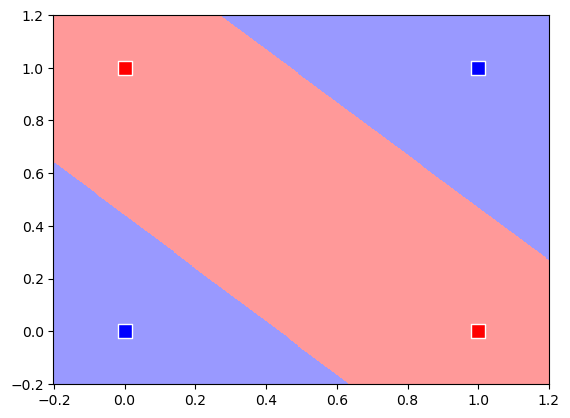
\includegraphics[height=0.6\linewidth]{Images/xor01}
				\label{fig:xor01}
			\end{figure}	
		\end{column}
	\end{columns}

\end{frame}

\begin{frame}{Porte OU EXCLUSIF - Interprétation}
	\begin{columns}
		\begin{column}{0.4\textwidth}
			\begin{table}
				\centering
				% \arraystretch permet d'aérer un peu les lignes du tableau
				\renewcommand{\arraystretch}{1.3} 
				\begin{tabular}{|c|c|c|c|c|}
					\hline
					%			% --- LE HEADER COLORÉ ---
					\rowcolor{blue!80!black} % Un fond bleu foncé
					\textcolor{white}{\textbf{$x_1$}} & 
					\textcolor{white}{\textbf{$x_2$}} & 
					\textcolor{white}{\textbf{$h_1$}} & 
					\textcolor{white}{\textbf{$h_2$}} & 
					\textcolor{white}{\textbf{$\hat{y}$}} \\
					\hline
					%			% --- LES DONNÉES ---
					0 & 0 & 1 & 1 & 0 \\
					\hline
					0 & 1 & 0 & 1 & 1 \\
					\hline
					1 & 0 & 0 & 1 & 1 \\
					\hline
					1 & 1 & 0 & 0 & 0 \\
					\hline
				\end{tabular}
			\end{table}
		\end{column}
		\begin{column}{0.6\textwidth}
			Quelle est l'opération logique réalisée par:
			\begin{itemize}
				\item Le premier neurone de la couche cachée ?
				\item Le second neurone de la couche cachée ?
				\item Le neurone de la couche de sortie ?
			\end{itemize}
		\end{column}
	\end{columns}

	\pause
	\vspace{0.3cm}
	
	\begin{itemize}
		\item Le premier neurone de la couche cachée réalise un NON OU:
		\begin{equation*}
			x_1, x_2 \mapsto \neg \left(x_1 \lor x_2\right)
		\end{equation*}
		\item Le second neurone de la couche cachée réalise un NON ET:
		\begin{equation*}
			x_1, x_2 \mapsto \neg \left(x_1 \land x_2\right)
		\end{equation*}
		\item Le neurone de la couche de sortie réalise un ET NON: 
		\begin{equation*}
			h_1, h_2 \mapsto h_2 \land \left(\neg h_1 \right)
		\end{equation*}
	\end{itemize}

\end{frame}

\begin{frame}{Porte OU EXCLUSIF - Vérification}
	Le réseau de neurone réalise donc l'opération:
	
	\begin{equation*}
		\begin{aligned}
			\hat{y} 
			&= h_2 \land \left(\neg h_1 \right) \\
			&= \left(\neg \left(x_1 \land x_2\right)\right) \land \neg \left( \neg \left(x_1 \lor x_2\right) \right) \\
			&= \left(\neg \left(x_1 \land x_2\right)\right) \land \left(x_1 \lor x_2\right) \\
			&= x_1 \oplus x_2
		\end{aligned}
	\end{equation*}
	
	C'est bien une opération de OU EXCLUSIF qui est réalisée. Il y a plusieurs solutions. Par exemple, le premier neurone, au lieu d'apprendre un NON OU, aurait pu apprendre un simple OU. Le neurone de sortie aurait alors dû apprendre un ET.
	
	\vspace{0.3cm}
	
	Pourquoi n'apprend-il pas la solution la plus \textit{simple} ?
\end{frame}

\begin{frame}{Porte OU EXCLUSIF - Un travail d'équipe !}
	Chaque porte \textit{codée} par le réseau de neurone est linéairement séparable. Mais la combinaison ne l'est pas:
	\begin{columns}
		\begin{column}{0.33\textwidth}
			\begin{figure}
				\centering
				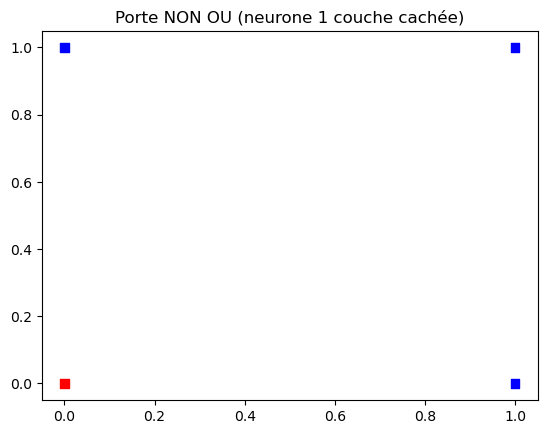
\includegraphics[height=0.85\linewidth]{Images/xor02}
				\label{fig:xor02}
			\end{figure}				
		\end{column}
		\begin{column}{0.33\textwidth}
			\begin{figure}
				\centering
				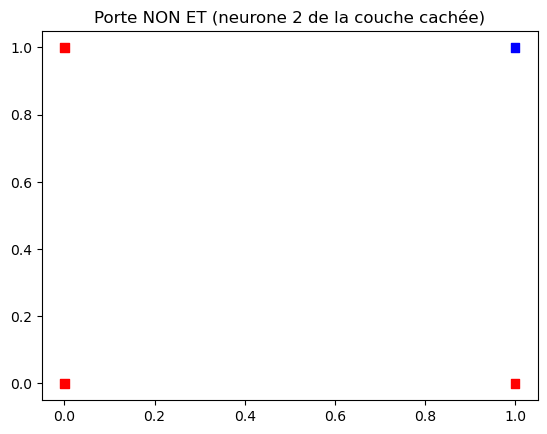
\includegraphics[height=0.85\linewidth]{Images/xor03}
				\label{fig:xor03}
			\end{figure}				
		\end{column}
				\begin{column}{0.33\textwidth}
			\begin{figure}
				\centering
				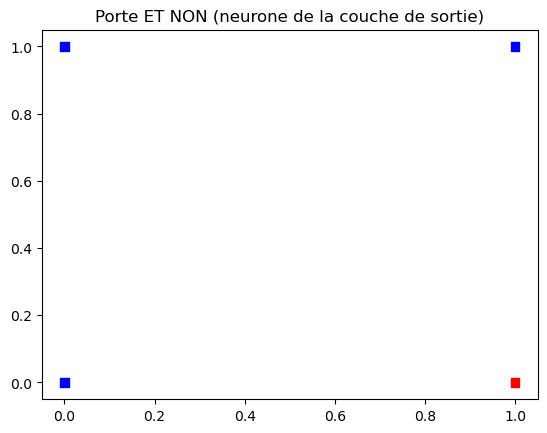
\includegraphics[height=0.85\linewidth]{Images/xor04}
				\label{fig:xor04}
			\end{figure}				
		\end{column}
	\end{columns}
	Le réseau de neurones se comporte comme une équipe. Chaque membre réalise une opération simple. Et c'est en combinant \textbf{non-linéairement} les deux neurones de la couche cachée grâce à la fonction d'\textbf{activation} que le réseau parvient à séparer correctement un problème non-linéaire.
\end{frame}

\begin{frame}{Porte OU EXCLUSIF - Visualisation}
	On peut visualiser l'\textbf{espace latent}. C'est l'espace généré par la première couche de neurones, c'est à dire l'espace formé par $h_1$ et $h_2$ pour l'ensemble des données d'apprentissage:
	
	\begin{columns}
		\begin{column}{0.4\textwidth}
			\begin{figure}
				\centering
				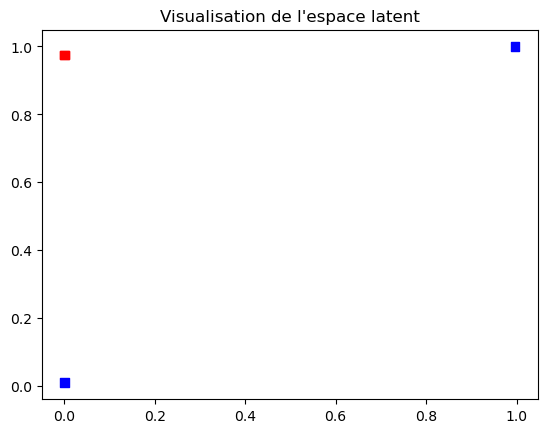
\includegraphics[height=0.9\linewidth]{Images/xor05}
				\label{fig:xor05}
			\end{figure}
		\end{column}	
		\begin{column}{0.6\textwidth}
			\begin{itemize}
				\item Dans l'espace latent, le problème est bien linéairement séparable. C'est pour cela que le neurone de la couche cachée arrive à reproduire la fonction OU EXCLUSIF.
				\item La couche cachée à \textit{tordu}, ou déformé non-linéairement l'espace, afin de rendre le problème linéairement séparable. La couche cachée a ainsi effectué une \textbf{simplification} du problème.
			\end{itemize}
		\end{column}
	\end{columns}
	
\end{frame}

\subsection[Fonctions d'activation]{Fonctions d'activation}

\begin{frame}{Choix des fonctions d'activation}
	Il est également possible d'utiliser des fonctions d'\textbf{activation} (aussi appelées fonctions \textbf{non-linéaires}) différentes à chaque couche.
	\begin{itemize}
		\item Le choix de la fonction d'activation sur la couche de sortie est généralement dicté par la nature du problème. Dans le cadre d'une \textbf{classification binaire}, la sortie $Y$ représente des probabilités, utiliser une fonction \textbf{logistique} est alors naturel.
		\pause
		\item Pour une classification multi-classe, utiliser une fonction \textbf{softmax} en sortie est un choix très pertinent. 
		\pause
		\item Pour un problème de \textbf{régression}, il n'y a en général pas de fonction d'activation sur la couche de sortie. Un réseau à une couche de neurones avec un neurone est donc \textbf{strictement} équivalent à la formulation mathématique d'une \textbf{régression linéaire}.
		\pause
		\item Pour les couches cachées, historiquement 3 fonctions se sont particulièrement distinguées: la fonction \textbf{logistique}, la \textbf{tangente hyperbolique} et la fonction linéaire rectifiée \textbf{ReLU}.
	\end{itemize}
\end{frame}

\begin{frame}{Représentation graphique des fonctions d'activation}
	\begin{alertblock}{Représentation graphique des fonctions d'activation}
		Les représentations graphiques de réseaux de neurones montrent souvent une fonction \textbf{sigmoïde} pour les fonctions d'activation par habitude. Il faut se tourner vers la définition mathématique des fonctions d'activation pour chaque couche. Leur représentation graphique reste \textbf{conceptuelle}.	
	\end{alertblock}
\end{frame}

\begin{frame}{Fonction logistique}
	\begin{block}{Fonction logistique}
		La fonction \textbf{logistique} est une fonction $\sigma: \R \to ]0, 1[$ définie comme suit:
		
		\begin{equation*}
			\sigma: z \mapsto \frac{1}{1 + e^{-z}}
		\end{equation*}
		
		Elle est un remplaçant naturel, et dérivable, de la fonction de Heaviside du Perceptron originel. Elle s'utilise généralement sur la couche de sortie des réseaux de neurones pour des problèmes de \textbf{classification binaire}. Elle s'utilise également dans les couches cachées.
	\end{block}
	
	\begin{figure}
		\centering
		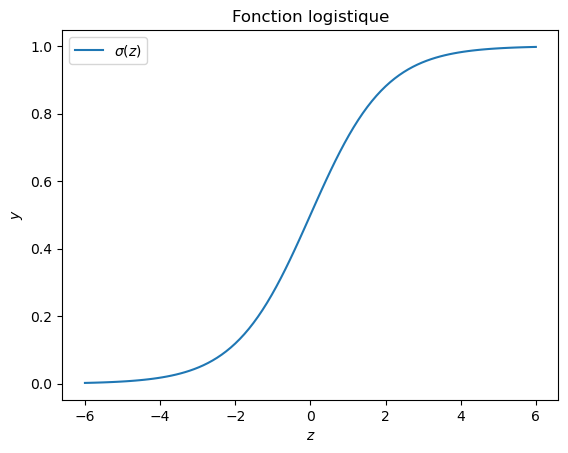
\includegraphics[height=0.25\linewidth]{Images/nonlinearites02}
		\label{fig:nonlinearites02}
	\end{figure}	
\end{frame}

\begin{frame}{Fonction softmax}
	\begin{block}{Fonction softmax}
		La fonction \textbf{softmax} est une fonction $\operatorname{softmax}: \R^p \to ]0, 1[^p$ définie comme suit:
		
		\begin{equation*}
			\operatorname{softmax}: z_j \mapsto \frac{e^{z_j}}{\sum_{i=1}^{p} e^{z_j}} \; \forall \; j = 1, 2, \cdots, p
		\end{equation*}
		
		C'est une généralisation de la fonction logistique pour des problèmes de \textbf{classification multi-classe} utilisée exclusivement sur la couche de sortie. Elle dispose de la propriété suivante:
		
		\begin{equation*}
			\sum_{i=1}^p \operatorname{softmax}\left(z_i\right) = 1
		\end{equation*}
	\end{block}
\end{frame}

\begin{frame}{Fonction softmax et stabilité numérique}
	\begin{block}{Version numériquement stable de la fonction softmax}
		La fonction \textbf{softmax} décrite précédemment n'est pas numériquement stable. Dans les programmes informatiques on préfère la définition suivante, équivalente:
				
		\begin{equation*}
			\operatorname{softmax}: z_j \mapsto \frac{e^{z_j - z_{\text{max}}}}{\sum_{i=1}^{p} e^{z_j - z_{\text{max}}}} \; \forall \; j = 1, 2, \cdots, p
		\end{equation*}
		
		Avec $z_{\text{max}}$, la valeur maximale des entrées $z$:

		\begin{equation*}
			z_{\text{max}} = \underset{j}{\max{\left(z_j\right)}} \; \text{;} \; j = 1, 2, \dots p
		\end{equation*}

		Cette définition limite les valeurs prises par les exponentielles des $z_j$.
	\end{block}
\end{frame}


\begin{frame}{Fonction tangente hyperbolique}
	\begin{block}{Fonction tangente hyperbolique}
		La fonction \textbf{tangente hyperbolique} est une fonction $\tanh: \R \to ]-1, 1[$ définie comme suit:
		
		\begin{equation*}
			\tanh: z \mapsto \frac{1 - e^{-2 z}}{1 + e^{- 2 z}}
		\end{equation*}
		
		Elle est extrêmement similaire à la fonction logistique mais prend valeur dans $]-1, 1[$. Elle est la fonction d'activation \textbf{historique} des réseaux de neurones \textbf{denses} simples.
	
	\end{block}

	\begin{figure}
		\centering
		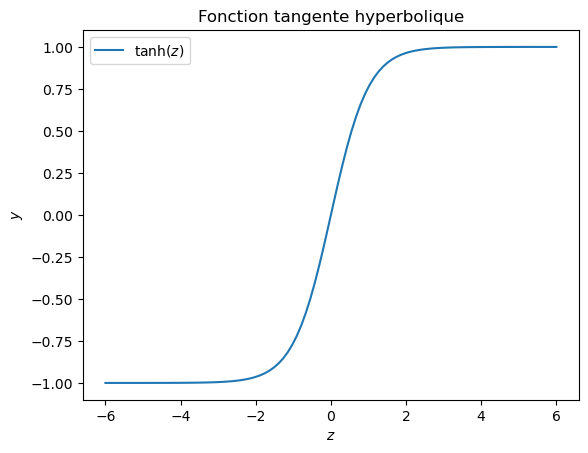
\includegraphics[height=0.25\linewidth]{Images/nonlinearites03}
		\label{fig:nonlinearites03}
	\end{figure}		
\end{frame}

\begin{frame}{Fonction linéaire rectifiée}
	\begin{block}{Fonction linéaire rectifiée: ReLU}
		La fonction \textbf{linéaire rectifiée} ou \textbf{ReLU} est une fonction $\operatorname{ReLU}: \R \to [0, +\infty[$ définie comme suit:
		
		\begin{equation*}
			\operatorname{ReLU}: z \mapsto \begin{cases}
				z & \text{si } \; z > 0 \\
				0 & \text{sinon}
			\end{cases}
		\end{equation*}
		
		Bien qu'elle soit non dérivable en 0, elle s'est imposée comme la fonction par défaut des réseaux de neurones complexes ou profonds.
		
	\end{block}
	
	\begin{figure}
		\centering
		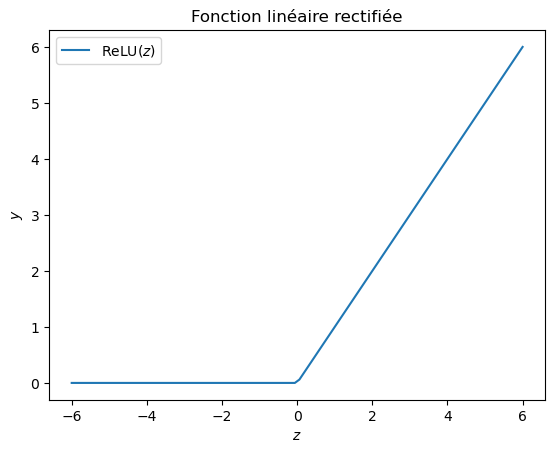
\includegraphics[height=0.3\linewidth]{Images/nonlinearites04}
		\label{fig:nonlinearites04}
	\end{figure}		
\end{frame}

\begin{frame}{Choix de la fonction d'activation des couches cachées}
	Pour les couches cachées:
	\begin{itemize}
		\item Le choix de la fonction d'activation constitue un \textbf{hyper-paramètre} du réseau de neurone.
		\pause
		\item Son choix résulte généralement d'une processus de sélection utilisant une \textbf{validation croisée}.
		\pause
		\item ReLU fonctionne généralement mieux sur les modèles disposant de nombreuses couches et de nombreux neurones par couche.
		\pause
		\item La fonction logistique et la tangente hyperbolique performent davantage sur des réseaux de neurones simples. Le choix entre l'une ou l'autre peut dépendre du choix de standardisation ou normalisation des données d'entrée.
	\end{itemize}
\end{frame}

\begin{frame}{Augmentation des données vs architecture du réseau}
	Avec les algorithmes de régressions linéaire et logistique, nous avons vu que pour résoudre un problème non-linéaire il fallait passer par une fonction d'augmentation $\Phi: \mathcal{X} \to \tilde{\mathcal{X}}$ faisant apparaitre des combinaisons non-linéaires des caractéristiques d'entrée $X$.
	
	\vspace{0.5cm}
	\pause
	
	Pour les réseaux de neurones, la capacité à traiter des problèmes non-linéaires repose sur:
	\begin{itemize}
		\item Le choix de la fonction d'activation: la source de non-linéarité.
		\item Le choix du nombre de couches.
		\item Le choix du nombre de neurones par couches.
	\end{itemize}
	
	\vspace{0.5cm}
	\pause
	
	Quelle approche est la plus puissante ? Laquelle privilégier ?
	
\end{frame}

\begin{frame}{Augmentation des données vs architecture du réseau}
	En pratique, \textit{les deux}:
	
	\begin{itemize}
		\item Le choix de la fonction d'augmentation $\Phi$ repose en général sur une \textbf{expertise} du domaine. Ce processus est appelé ingénierie des caractéristiques ou \textbf{feature engineering}. Si on sait que la variable de sortie d'un problème de régression dépend d'une caractéristique d'entrée au carré, il vaut généralement mieux faire apparaitre cette caractéristique au carré en entrée plutôt que de laisser le réseau de neurones \textbf{reconstruire} ce type de relation.
		\pause
		\item Les relations entre les entrées et les sorties peuvent être si complexes qu'une expertise du domaine peut être insuffisante pour établir clairement ces relations. Les réseaux de neurones permettent alors de les \textbf{découvrir} pour nous.
		\pause
		\item La \textbf{simplicité} doit primer. Un \textbf{feature engineering} \textit{malin} permet de réduire la complexité du réseau de neurones. Pour une quantité de données limitée, cela peut réduire la \textbf{variance} du modèle. En fournissant des éléments de réponse basés sur une expertise métier, le \textbf{feature engineering} peut aussi permettre de réduire le \textbf{biais}.
	\end{itemize}	
\end{frame}

\begin{frame}{Passe avant dans une couche de neurones}
	
	\begin{block}{Passe avant dans une couche de neurones}
		Pour résumer une \textbf{passe avant} dans une couche d'une réseau de neurones dense lorsqu'il fait une \textbf{prédiction}:
		
		\begin{equation*}
			X \mapsto \logistic{X W + b}
		\end{equation*} 
		
		Il s'agit donc de la combinaison entre une opération \textbf{linéaire} suivie d'une \textbf{non-linéarité}.		
	\end{block}
	
	\vspace{0.3cm}
	
	Note: dans la suite de ce cours on notera, de manière générique, $\sigma$ toute fonction d'activation (logistique, tangente hyperbolique ou ReLU).

\end{frame}
